\documentclass{beamer}
\usetheme{Frankfurt}
\usepackage{textcomp}
\usepackage{german}
\usepackage{tikz}
\usepackage{pgfplots}
\usepackage{booktabs}% http://ctan.org/pkg/booktabs
\newcommand{\tabitem}{~~\llap{\textbullet}~~}
\usetikzlibrary{automata,positioning}
\usetikzlibrary{arrows,automata,shapes,calc}
\setbeamertemplate{navigation symbols}{}%remove navigation symbols
%\setbeamercolor{normal text}{fg=white,bg=black!90}
\setbeamercolor{normal text}{fg=black!90,bg=white}
\setbeamercolor{structure}{fg=darkgray!90,bg=white}

\setbeamercolor{alerted text}{fg=red!85!black}

%\setbeamercolor{item projected}{use=item,fg=black,bg=item.fg!35}

%\setbeamercolor*{palette primary}{use=structure,fg=structure.fg}
%\setbeamercolor*{palette secondary}{use=structure,fg=structure.fg!95!black}
%\setbeamercolor*{palette tertiary}{use=structure,fg=structure.fg!90!black}
%\setbeamercolor*{palette quaternary}{use=structure,fg=structure.fg!95!black,bg=black!80}

%\setbeamercolor*{framesubtitle}{fg=white}
%
%\setbeamercolor*{block title}{parent=structure,bg=black!60}
%\setbeamercolor*{block body}{fg=black,bg=black!10}
%\setbeamercolor*{block title alerted}{parent=alerted text,bg=black!15}
%\setbeamercolor*{block title example}{parent=example text,bg=black!15}

\AtBeginSection []{
	\begin{frame}
		\frametitle{Inhaltsverzeichnis}
		\tableofcontents[currentsection,subsubsectionstyle={show/show/show/shaded}]
	\end{frame}
}

\AtBeginSubsection []{
	\begin{frame}
		\frametitle{Inhaltsverzeichnis}
		\tableofcontents[currentsection,subsectionstyle={show/shaded/shaded}]
	\end{frame}
}

\AtBeginSubsubsection []{
	\begin{frame}
		\frametitle{Inhaltsverzeichnis}
		\tableofcontents[currentsection,subsectionstyle={show/shaded/shaded},subsubsectionstyle={show/shaded/shaded/shaded}]
	\end{frame}
}

\begin{document}
\title{Evaluierung der Cache-Hierarchie eines nachrichtengekoppelten Manycore-Prozessors}
\author{Dominik Walter}

\date{\today}

\frame{\titlepage}


\frame{\frametitle{Inhaltsverzeichnis}\tableofcontents}




\section{RCMC-Architektur}
\frame{\frametitle{RCMC-Architektur}
	
\begin{figure}[htbp]
	\centering
	\begin{minipage}{0.5\textwidth}
		\includegraphics[width=1\textwidth]{chip.png}
		
	\end{minipage}
	\caption{Aufbau der RCMC-Architektur}
	\label{f:chip}
\end{figure}
\pause
\begin{block}{ Eigenschaften}
\begin{table}[htbp]
	\begin{tabular}{l|l}
		Original & Erweiterung \\\hline

		\tabitem lokaler Speicher
		& 
		\tabitem lokaler Cache
		\\
		\tabitem kein Hauptspeicher
		& 
		\tabitem gemeinsamer Hauptspeicher
		\\
		\tabitem Zugriffszeit immer 1 Takt
		& 
		\tabitem realistische Zugriffszeit
		\\
		
		\hline
		
		
	\end{tabular}
\end{table}
\end{block}


}

\section{Evaluierung}
\subsection{Simulator}
\frame{\frametitle{Simulator}
		
	\begin{columns}
		\begin{column}{.5\textwidth}
			\begin{block}{Original}
				\begin{figure}
					\begin{minipage}{0.9\textwidth}
						\includegraphics[width=1\textwidth]{simNoCache.png}
					\end{minipage}
				\end{figure}
			\end{block}
		\end{column}
		\pause
		\begin{column}{.5\textwidth}
			\begin{block}{Mit Speichersystem}
				\begin{figure}
					\begin{minipage}{0.9\textwidth}
						\includegraphics[width=1\textwidth]{simCache.png}
					\end{minipage}
				\end{figure}
			\end{block}
		\end{column}
	\end{columns}

	
}
\subsection{Tests}
\frame{\frametitle{Tests}
	\begin{block}{Prozessor}
		\tabitem 4x4 Kerne \\
		\tabitem RCMC-Manycore 
	\end{block}	
	\pause
	\begin{block}{Hauptspeicher}
		\tabitem 1 Channel \\
		\tabitem 1 Queue \\
		\tabitem Hohe Zugriffszeit
	\end{block}	
	\pause
	\begin{block}{Benchmarks}
		\tabitem Integer Sort (IS) \\
		\tabitem Data Traffic (DT) \\
		\tabitem Conjugate Gradient (CG) \\
	\end{block}		
}
\subsubsection{Schreibstrategie}
\frame{\frametitle{Schreibstrategie}
	\begin{block}{Problematik}
		\tabitem Wann werden die Eintr\"age im Hauptspeicher aktualisiert?
	\end{block}	
	\pause
	\begin{block}{L\"osung I: Write-Through}
		\tabitem Daten werden immer direkt in den RAM schreiben \\
		\tabitem Im Speicher steht immer der aktuelle Wert \\
	\end{block}	
	\pause
	\begin{block}{L\"osung II: Write-Back}
		\tabitem Erst bei einer Verdr\"angung wird zur\"uckgeschrieben\\
		\tabitem Weniger Traffic \\
		\tabitem Aufw\"andiger zu Implementieren
	\end{block}	
	
}
\frame{\frametitle{Schreibstrategie}
	\begin{block}{Problematik}
		\tabitem Wird beim Schreiben der Eintrag in den Cache geladen?
	\end{block}	
	\pause
	\begin{block}{L\"osung I: Write-Allocate}
		\tabitem Bei einem Schreibzugriff wird der Eintrag in den Cache geladen \\
		\tabitem Nur mit Write-Back sinnvoll \\
		\tabitem Folgen auf einen Schreibzugriff weitere Zugriffe, so befindet sich der Eintrag bereits im Cache
	\end{block}	
	\pause
	\begin{block}{L\"osung II: Write-Non-Allocate}
		\tabitem Bei einem Schreibzugriff wird der Eintrag nicht in den Cache geladen \\
		\tabitem Eventuell unn\"otiger Eintrag wird nicht in den Cache geladen
	\end{block}			
}

\frame{\frametitle{Schreibstrategie}
	
	\begin{figure}[htbp]
		\begin{minipage}{1\textwidth}
			% legend
			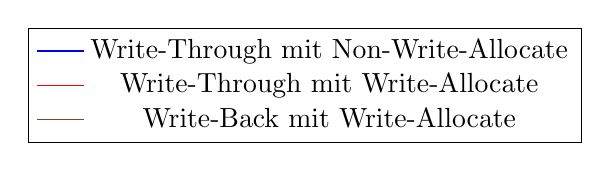
\begin{tikzpicture}
			\begin{axis}[
			width=1.075\textwidth,
			height=0.2\textwidth,
			%		xlabel={Tests (IS)},
			hide axis,
			%		legend style={at={(0.5,1.05)},anchor=south},
			symbolic x coords={0}
			]
			
			
			\addplot +[mark=] coordinates {
				(0,0)
			};
			
			\addplot +[mark=] coordinates {
				(0,0)
			};
			
			\addplot +[mark=] coordinates {
				(0,0)
			};
			\legend{Write-Through mit Non-Write-Allocate, Write-Through mit Write-Allocate, Write-Back mit Write-Allocate}
			\end{axis}
			\end{tikzpicture}
		\end{minipage}
		
		\begin{minipage}{0.325\textwidth}
			\begin{tikzpicture}
			\begin{semilogyaxis}[
			width=1.05\textwidth,
			ylabel={Takte},
			xlabel={Offset},
			legend style={at={(0.5,1.05)},anchor=south,legend
				columns=-1},
			symbolic x coords={1, 2, 3, 4, 5, 6, 7, 8, 9, 10, 11, 12, 13, 14}
			]
			
			
			\addplot +[mark=] coordinates {				
				(1, 501879639) (2, 551922692) (3, 549621613) (4, 457833044) (5, 411925249) (6, 388883598) (7, 377369885) (8, 371635052) (9, 368797614) (10, 367360978) (11, 366737522) (12, 376469232) (13, 646453790) (14, 1273306679)
				
				
			};
			
			\addplot +[mark=] coordinates {
				(1, 452144048) (2, 525750431) (3, 537489804) (4, 451257137) (5, 408602109) (6, 387519450) (7, 377129855) (8, 371888758) (9, 369409407) (10, 367942408) (11, 369235824) (12, 387761234) (13, 679510070) (14, 1631803741) 
			};
			
			
			
			\addplot +[mark=] coordinates {
				(1, 317210263) (2, 400796096) (3, 416304011) (4, 217995453) (5, 123933576) (6, 86812625) (7, 76601101) (8, 70491878) (9, 68682456) (10, 69442187) (11, 77117298) (12, 159577563) (13, 815815632) (14, 2007413606)
			};
			
			\end{semilogyaxis}
			\end{tikzpicture}
		\end{minipage}
		\begin{minipage}{0.325\textwidth}
			\begin{tikzpicture}
			\begin{semilogyaxis}[
			width=1.05\textwidth,
			ylabel={lad. Bytes},
			xlabel={Offset},
			legend style={at={(0.5,1.05)},anchor=south,legend
				columns=-1},
			symbolic x coords={1, 2, 3, 4, 5, 6, 7, 8, 9, 10, 11, 12, 13, 14}
			]
			
			
			\addplot +[mark=] coordinates {
				(1, 525792) (2, 1297444) (3, 2581784) (4, 2588624) (5, 2603616) (6, 2629504) (7, 2675456) (8, 2763264) (9, 3061760) (10, 3670016) (11, 5890048) (12, 62832640) (13, 4207550464) (14, 32125763584)
				
			};
			
			\addplot  +[mark=] coordinates {
				(1, 881778) (2, 2058464) (3, 4268784) (4, 4335024) (5, 4547968) (6, 5392512) (7, 7812224) (8, 11814400) (9, 20312064) (10, 37578752) (11, 81674240) (12, 396058624) (13, 7702872064) (14, 57712394240) 
				
			};
			
			\addplot +[mark=] coordinates {
				(1, 846622) (2, 2047464) (3, 4256552) (4, 4310256) (5, 4558848) (6, 5382208) (7, 7823616) (8, 11824896) (9, 20318208) (10, 37588992) (11, 81770496) (12, 396103680) (13, 7702872064) (14, 57712001024) 
			};
			
			
			%		\legend{}
			\end{semilogyaxis}
			\end{tikzpicture}
		\end{minipage}
		\begin{minipage}{0.325\textwidth}
			\begin{tikzpicture}
			\begin{semilogyaxis}[
			width=1.05\textwidth,	
			ylabel={schr. Bytes},
			xlabel={Offset},
			legend style={at={(0.5,1.05)},anchor=south,legend
				columns=-1},
			symbolic x coords={1, 2, 3, 4, 5, 6, 7, 8, 9, 10, 11, 12, 13, 14}
			]
			
			
			\addplot +[mark=] coordinates {
				(1, 6247136) (2, 6247136) (3, 6247136) (4, 6247136) (5, 6247136) (6, 6247136) (7, 6247136) (8, 6247136) (9, 6247136) (10, 6247136) (11, 6247136) (12, 6247136) (13, 6247136) (14, 6247136) 
				
				
			};
			
			\addplot +[mark=] coordinates {
				(1, 6247136) (2, 6247136) (3, 6247136) (4, 6247136) (5, 6247136) (6, 6247136) (7, 6247136) (8, 6247136) (9, 6247136) (10, 6247136) (11, 6247136) (12, 6247136) (13, 6247136) (14, 6247136) 
			};
			
			\addplot +[mark=] coordinates {
				(1, 444248) (2, 924656) (3, 1898256) (4, 1961376) (5, 2170592) (6, 2993472) (7, 5378560) (8, 9313536) (9, 17534464) (10, 34295808) (11, 76449792) (12, 351207424) (13, 789258240) (14, 789258240) 
				
			};
			
			%		\legend{}
			\end{semilogyaxis}
			\end{tikzpicture}
		\end{minipage}
		\caption[Schreibstrategie]{Vergleich zwischen verschiedenen Schreibstrategien}
		\label{f:IS_WB_WA}
	\end{figure}
}
\subsubsection{Cache-Line Gr\"o{\ss}e}
\frame{\frametitle{Cache-Line Gr\"o{\ss}e}
	\begin{block}{Problematik}
		\tabitem Wie gro\ss{} sollte eine Cache-Line sein?\\
	\end{block}	
	\pause
	\begin{block}{L\"osung I: Kleine Cache-Line}
		\tabitem Bei einer Verdr\"angung werden weniger Daten ersetzt\\
		\tabitem Schlechte Ausnutzung der Lokalit\"ats-Eigenschaft\\	
	\end{block}	
	\pause
	\begin{block}{L\"osung II: Gro\ss{}e Cache-Line}
		\tabitem Bessere Ausnutzung der Lokalit\"ats-Eigenschaft\\
		\tabitem Bei Cache-Misses m\"ussen mehr Daten geladen werden\\
		
	\end{block}	
}
\frame{\frametitle{Cache-Line Gr\"o{\ss}e}
	\begin{figure}[htbp]
		\begin{minipage}{1\textwidth}
			% legend
			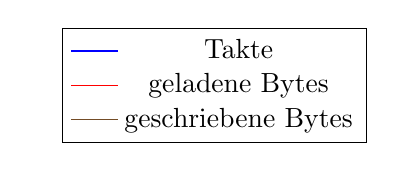
\begin{tikzpicture}
			\begin{axis}[
			width=0.87\textwidth,
			height=0.2\textwidth,
			%		xlabel={Tests (IS)},
			hide axis,
			%		legend style={at={(0.5,1.05)},anchor=south},
			symbolic x coords={0}
			]
			
			% cycle
			\addplot +[mark=] coordinates {
				(0,0)
			};
			% Load
			\addplot +[mark=] coordinates {
				(0,0)
			};
			% Store
			\addplot +[mark=] coordinates {
				(0,0)
			};
			\legend{Takte, geladene Bytes, geschriebene Bytes}
			\end{axis}
			\end{tikzpicture}
		\end{minipage}
		%IS
		\begin{minipage}{0.325\textwidth}
			\begin{tikzpicture}
			\begin{semilogyaxis}[
			width=1.15\textwidth,
			xlabel={Tests (IS)},
			legend style={at={(0.5,1.05)},anchor=south,
				columns=-1},
			symbolic x coords={29, 30, 31, 32, 33, 34, 35, 36, 37, 38, 39, 40, 41, 42}
			]
			% cycle
			\addplot +[mark=] coordinates {
				(29, 317210263) (30, 400796096) (31, 416304011) (32, 217955453) (33, 123933576) (34, 86812625) (35, 76601101) (36, 70491878) (37, 68682456) (38, 69442187) (39, 77117298) (40, 159577563) (41, 815815632) (42, 2007413606)
				
				
			};
			% Load
			\addplot +[mark=] coordinates {
				(29, 846622) (30, 2047464) (31, 4256552) (32, 4310256) (33, 4558848) (34, 5382208) (35, 7823616) (36, 11824896) (37, 20318208) (38, 37588992) (39, 81770496) (40, 396103680) (41, 7702872064) (42, 57712001024)
			};
			% Store
			\addplot +[mark=] coordinates {
				(29, 444248) (30, 924656) (31, 1898256) (32, 1961376) (33, 2170592) (34, 2993472) (35, 5378560) (36, 9313536) (37, 17534464) (38, 34295808) (39, 76449792) (40, 351207424) (41, 5084225536) (42, 12794134528)
			};
			
			%		\legend{}
			\end{semilogyaxis}
			\end{tikzpicture}
		\end{minipage}
		%DT
		\begin{minipage}{0.325\textwidth}
			\begin{tikzpicture}
			\begin{semilogyaxis}[
			width=1.15\textwidth,
			xlabel={Tests (DT)},
			legend style={at={(0.5,1.05)},anchor=south,legend
				columns=-1},
			symbolic x coords={29, 30, 31, 32, 33, 34, 35, 36, 37, 38, 39, 40, 41, 42}
			]
			% cycle
			\addplot +[mark=] coordinates {
				(29, 8395384) (30, 14892369) (31, 13281091) (32, 7195049) (33, 4241378) (34, 2793643) (35, 2035421) (36, 1712928) (37, 1664873) (38, 1590158) (39, 1652294) (40, 1889231) (41, 2705778) (42, 24402410)
				
				
			};
			% load
			\addplot +[mark=] coordinates {
				(29, 25106) (30, 78140) (31, 139064) (32, 142160) (33, 146912) (34, 154496) (35, 167936) (36, 203776) (37, 515072) (38, 987136) (39, 2684928) (40, 8577024) (41, 43253760) (42, 947961856)
			};
			% store
			\addplot +[mark=] coordinates {
				(29, 4828) (30, 30116) (31, 59888) (32, 60512) (33, 61024) (34, 62528) (35, 64256) (36, 71168) (37, 96768) (38, 162816) (39, 421888) (40, 2301952) (41, 16580608) (42, 209928192)
			};
			
			%		\legend{}
			\end{semilogyaxis}
			\end{tikzpicture}
		\end{minipage}
		% CG
		\begin{minipage}{0.325\textwidth}
			\begin{tikzpicture}
			\begin{semilogyaxis}[
			width=1.15\textwidth,
			xlabel={Tests (CG)},
			legend style={at={(0.5,1.05)},anchor=south,legend
				columns=-1},
			symbolic x coords={29, 30, 31, 32, 33, 34, 35, 36, 37, 38, 39, 40, 41, 42}
			]
			% cycle
			\addplot +[mark=] coordinates {
				(29, 2724375064) (30, 2857542765) (31, 2432535321) (32, 1195428620) (33, 609186226) (34, 322637809) (35, 184092073) (36, 117716322) (37, 97009862) (38, 93612405) (39, 128049787) (40, 781456372) (41, 4517561310) (42, 10749622007) 
				
				
				
			};
			% load
			\addplot +[mark=] coordinates {
				(29, 6893106) (30, 14156188) (31, 23541760) (32, 23305216) (33, 23486432) (34, 23961152) (35, 24885760) (36, 28753920) (37, 32977408) (38, 43620352) (39, 120666112) (40, 4966662144) (41, 48409001984) (42, 273045979136) 
				
			};
			% store
			\addplot +[mark=] coordinates {
				(29, 1310812) (30, 2973164) (31, 6532624) (32, 6593504) (33, 6729056) (34, 6941632) (35, 7389952) (36, 8198400) (37, 10003968) (38, 15730688) (39, 74698752) (40, 966553600) (41, 10998521856) (42, 29835476992)
			};
			
			%		\legend{}
			\end{semilogyaxis}
			\end{tikzpicture}
		\end{minipage}
		\caption[Cache-Größe]{F\"ur gr\"o\ss{}ere \textit{Cache-Lines} steigt der \textit{Traffic}, w\"ahrend die Takte bei Test 38 minimal sind.}
	\end{figure}
}
\subsubsection{Assoziativit\"at}
\frame{\frametitle{Assoziativit\"at}
	\begin{block}{Problematik}
		\tabitem Wieviele Eintr\"age m\"ussen bei einem Zugriff verglichen werden?
	\end{block}	
	\pause
	\begin{block}{L\"osung I: Direkt-Abgebildet}
		\tabitem 1 Eintrag \\
		\tabitem Schlechte Ausnutzung des Cache-Speichers
		
	\end{block}	
	\pause
	\begin{block}{L\"osung II: n-Fach Satz-Assoziativ}
		\tabitem n Eintr\"age \\
		\tabitem Bessere Ausnutzung des Cache-Speichers
	\end{block}	
	\pause
	\begin{block}{L\"osung III: Voll-Assoziativ}
		\tabitem alle Eintr\"age  \\
		\tabitem Beste Ausnutzung des Cache-Speichers
	\end{block}	
	
}
\frame{\frametitle{Assoziativit\"at}
	\begin{figure}[htbp]
		\begin{minipage}{1\textwidth}
			% legend
			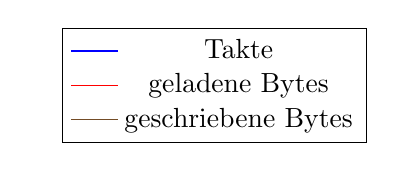
\begin{tikzpicture}
			\begin{axis}[
			width=0.87\textwidth,
			height=0.2\textwidth,
			%		xlabel={Tests (IS)},
			hide axis,
			%		legend style={at={(0.5,1.05)},anchor=south},
			symbolic x coords={0}
			]
			
			% cycle
			\addplot +[mark=] coordinates {
				(0,0)
			};
			% Load
			\addplot +[mark=] coordinates {
				(0,0)
			};
			% Store
			\addplot +[mark=] coordinates {
				(0,0)
			};
			\legend{Takte, geladene Bytes, geschriebene Bytes}
			\end{axis}
			\end{tikzpicture}
		\end{minipage}
		%IS
		\begin{minipage}{0.325\textwidth}
			\begin{tikzpicture}
			\begin{semilogyaxis}[
			width=1.15\textwidth,
			xlabel={Tests (IS)},
			legend style={at={(0.5,1.05)},anchor=south,
				columns=-1},
			symbolic x coords={43, 44, 45, 46, 47, 48}
			]
			% cycle
			\addplot +[mark=] coordinates {
				(43, 114179438) (44, 93820734) (45, 89977059) (46, 88366025) (47, 87675241) (48, 86812625)
			};
			% Load
			\addplot +[mark=] coordinates {
				(43, 8029056) (44, 5727168) (45, 5554176) (46, 5477184) (47, 5455872) (48, 5382208)
			};
			% Store
			\addplot +[mark=] coordinates {
				(43, 4434752) (44, 3340288) (45, 3143680) (46, 3066752) (47, 3043840) (48, 2993472)
			};
			
			%		\legend{}
			\end{semilogyaxis}
			\end{tikzpicture}
		\end{minipage}
		%DT
		\begin{minipage}{0.325\textwidth}
			\begin{tikzpicture}
			\begin{semilogyaxis}[
			width=1.15\textwidth,
			xlabel={Tests (DT)},
			legend style={at={(0.5,1.05)},anchor=south,legend
				columns=-1},
			symbolic x coords={43, 44, 45, 46, 47, 48}
			]
			% cycle
			\addplot +[mark=] coordinates {
				(43, 3198499) (44, 2842165) (45, 2803553) (46, 2795124) (47, 2793354) (48, 2793643)		
			};
			% load
			\addplot +[mark=] coordinates {
				(43, 257664) (44, 179200) (45, 161408) (46, 155584) (47, 154752) (48, 154496)
			};
			% store
			\addplot +[mark=] coordinates {
				(43, 74880) (44, 62464) (45, 63168) (46, 62720) (47, 62592) (48, 62528)
			};
			
			%		\legend{}
			\end{semilogyaxis}
			\end{tikzpicture}
		\end{minipage}
		% CG
		\begin{minipage}{0.325\textwidth}
			\begin{tikzpicture}
			\begin{semilogyaxis}[
			width=1.15\textwidth,
			xlabel={Tests (CG)},
			legend style={at={(0.5,1.05)},anchor=south,legend
				columns=-1},
			symbolic x coords={43, 44, 45, 46, 47, 48}
			]
			% cycle
			\addplot +[mark=] coordinates {
				(43, 491761891) (44, 343984939) (45, 323518729) (46, 324724453) (47, 323010929) (48, 322637809)
			};
			% load
			\addplot +[mark=] coordinates {
				(43, 49160320) (44, 26408832) (45, 24722048) (46, 24682496) (47, 24242944) (48, 23961152)	
			};
			% store
			\addplot +[mark=] coordinates {
				(43, 9056256) (44, 7277248) (45, 6890944) (46, 6917504) (47, 6929152) (48, 6941632)
			};
			
			%		\legend{}
			\end{semilogyaxis}
			\end{tikzpicture}
		\end{minipage}
		\caption[Assoziation]{Die Satzgr\"o\ss{}e hat kaum Einfluss auf die \textit{Benchmarks}}
	\end{figure}
	
}
\subsubsection{Cache Gr\"o{\ss}e}
\frame{\frametitle{Cache Gr\"o{\ss}e}
	\begin{block}{Problematik}
		\tabitem Wie gro\ss{} muss der Cache mindestens sein?\\
		\tabitem Gibt es eine maximale Gr\"o\ss{}e?
	\end{block}	
	\pause
	\begin{block}{L\"osung}
		\tabitem So gro\ss{} wie m\"oglich \\
		\tabitem Platz auf Chip ist begrenzt
	\end{block}	
}
\frame{\frametitle{Cache Gr\"o{\ss}e}
	
	\begin{figure}[htbp]
		\begin{minipage}{1\textwidth}
			% legend
			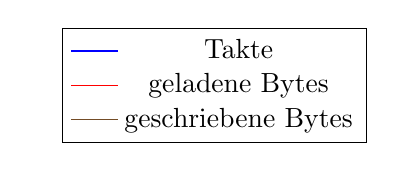
\begin{tikzpicture}
			\begin{axis}[
			width=0.87\textwidth,
			height=0.2\textwidth,
			%		xlabel={Tests (IS)},
			hide axis,
			%		legend style={at={(0.5,1.05)},anchor=south},
			symbolic x coords={0}
			]
			
			% cycle
			\addplot +[mark=] coordinates {
				(0,0)
			};
			% Load
			\addplot +[mark=] coordinates {
				(0,0)
			};
			% Store
			\addplot +[mark=] coordinates {
				(0,0)
			};
			\legend{Takte, geladene Bytes, geschriebene Bytes}
			\end{axis}
			\end{tikzpicture}
		\end{minipage}
		\begin{minipage}{0.325\textwidth}
			\begin{tikzpicture}
			\begin{semilogyaxis}[
			width=1.15\textwidth,
			xlabel={Tests (IS)},
			legend style={at={(0.5,1.05)},anchor=south,
				columns=-1},
			symbolic x coords={49, 50, 51, 52, 53, 54, 55, 56, 57, 58, 59, 60, 61, 62, 63, 64, 65, 66}
			]
			
			% cycle
			\addplot +[mark=] coordinates {
				(49, 2666401972) (50, 1655350773) (51, 1134468079) (52, 368942462) (53, 241151721) (54, 201882705) (55, 154281617) (56, 118212744) (57, 86812625) (58, 63209037) (59, 49212710) (60, 24307606) (61, 20384008) (62, 20384008) (63, 20384008) (64, 20384008) (65, 20384008) (66, 20384008) 
			};
			% Load
			\addplot +[mark=] coordinates {
				(49, 314189568) (50, 179611456) (51, 122839552) (52, 22461952) (53, 13668992) (54, 12034816) (55, 10109504) (56, 7439104) (57, 5382208) (58, 4283200) (59, 3399552) (60, 1880960) (61, 205120) (62, 205120) (63, 205120) (64, 205120) (65, 205120) (66, 205120)
			};
			% Store
			\addplot +[mark=] coordinates {
				(49, 49977088) (50, 48715136) (51, 40898880) (52, 11603392) (53, 10040704) (54, 8487040) (55, 6729280) (56, 4920832) (57, 2993472) (58, 2080384) (59, 1781184) (60, 1358656) (61, 0) (62, 0) (63, 0) (64, 0) (65, 0) (66, 0)
			};
			
			%		\legend{}
			\end{semilogyaxis}
			\end{tikzpicture}
		\end{minipage}
		%DT
		\begin{minipage}{0.325\textwidth}
			\begin{tikzpicture}
			\begin{semilogyaxis}[
			width=1.15\textwidth,
			xlabel={Tests (DT)},
			legend style={at={(0.5,1.05)},anchor=south,legend
				columns=-1},
			symbolic x coords={49, 50, 51, 52, 53, 54, 55, 56, 57, 58, 59, 60, 61, 62, 63, 64, 65, 66}
			]
			% cycle
			\addplot +[mark=] coordinates {
				(49, 29976733) (50, 16355440) (51, 5182833) (52, 4718114) (53, 4265411) (54, 3631693) (55, 3251336) (56, 2807356) (57, 2793643) (58, 2849619) (59, 2124843) (60, 1973707) (61, 1795986) (62, 1795986) (63, 1795986) (64, 1795986) (65, 1795986) (66, 1795986)
			};
			% load
			\addplot +[mark=] coordinates {
				(49, 5196352) (50, 2204224) (51, 723648) (52, 609920) (53, 519424) (54, 387200) (55, 295040) (56, 165376) (57, 154496) (58, 154496) (59, 95168) (60, 88000) (61, 88000) (62, 88000) (63, 88000) (64, 88000) (65, 88000) (66, 88000)
			};
			% store
			\addplot +[mark=] coordinates {
				(49, 820032) (50, 379968) (51, 180736) (52, 151808) (53, 130432) (54, 100416) (55, 82816) (56, 64512) (57, 62528) (58, 62016) (59, 16960) (60, 0) (61, 0) (62, 0) (63, 0) (64, 0) (65, 0) (66, 0)
			};
			
			%		\legend{}
			\end{semilogyaxis}
			\end{tikzpicture}
		\end{minipage}
		% CG
		\begin{minipage}{0.325\textwidth}
			\begin{tikzpicture}
			\begin{semilogyaxis}[
			width=1.15\textwidth,
			xlabel={Tests (CG)},
			legend style={at={(0.5,1.05)},anchor=south,legend
				columns=-1},
			symbolic x coords={49, 50, 51, 52, 53, 54, 55, 56, 57, 58, 59, 60, 61, 62, 63, 64, 65, 66}
			]
			% cycle
			\addplot +[mark=] coordinates {
				(49, 11674877548) (50, 6031780240) (51, 2735168694) (52, 1731761980) (53, 1509844945) (54, 999130516) (55, 570689949) (56, 372170512) (57, 322637809) (58, 306962807) (59, 287268517) (60, 85621314) (61, 83349583) (62, 83263345) (63, 83263345) (64, 83263345) (65, 83263345) (66, 83263345)
			};
			% load
			\addplot +[mark=] coordinates {
				(49, 1205323840) (50, 587957504) (51, 263618304) (52, 138372288) (53, 121423296) (54, 82495808) (55, 46764608) (56, 30401024) (57, 23961152) (58, 22416960) (59, 21514112) (60, 505600) (61, 313152) (62, 304256) (63, 304256) (64, 304256) (65, 304256) (66, 304256)
			};
			% store
			\addplot +[mark=] coordinates {
				(49, 116544896) (50, 110660864) (51, 77117184) (52, 20329472) (53, 17415808) (54, 11509440) (55, 10409088) (56, 7332160) (57, 6941632) (58, 5784448) (59, 4936704) (60, 223744) (61, 34304) (62, 0) (63, 0) (64, 0) (65, 0) (66, 0)
			};
			
			%		\legend{}
			\end{semilogyaxis}
			\end{tikzpicture}
		\end{minipage}
		\caption[Cache-Größe]{Stetige Verbesserung durch Vergr\"o\ss{}erung des Caches}
	\end{figure}
}
\subsubsection{Zugriffszeit}
\frame{\frametitle{Zugriffszeit}
	\begin{block}{Problematik}
		\tabitem Wann schnell muss der Cache sein um sich noch zu lohnen?\\
		\tabitem Ist ein kleiner schneller Cache besser als ein Gr\"o\ss{}erer?
	\end{block}	
	\pause
	\begin{block}{L\"osung I: Klein und Schnell}
		\tabitem K\"urzere Zugriffszeit\\
		\tabitem Niedrigere Hit-Rate		
	\end{block}	
	\pause
	\begin{block}{L\"osung II: Gro\ss{} und Langsam}
		\tabitem L\"angere Zugriffszeit \\
		\tabitem H\"ohere Hit-Rate
		
	\end{block}	
}
\frame{\frametitle{Zugriffszeit}
	\begin{figure}[htbp]
		\begin{minipage}{1\textwidth}
			% legend
			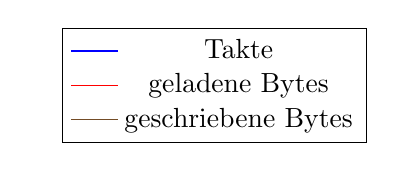
\begin{tikzpicture}
			\begin{axis}[
			width=0.87\textwidth,
			height=0.2\textwidth,
			%		xlabel={Tests (IS)},
			hide axis,
			%		legend style={at={(0.5,1.05)},anchor=south},
			symbolic x coords={0}
			]
			
			% cycle
			\addplot +[mark=] coordinates {
				(0,0)
			};
			% Load
			\addplot +[mark=] coordinates {
				(0,0)
			};
			% Store
			\addplot +[mark=] coordinates {
				(0,0)
			};
			\legend{Takte, geladene Bytes, geschriebene Bytes}
			\end{axis}
			\end{tikzpicture}
		\end{minipage}
		\begin{minipage}{0.325\textwidth}
			% IS
			\begin{tikzpicture}
			\begin{semilogyaxis}[
			width=1.15\textwidth,
			xlabel={Tests (IS)},
			legend style={at={(0.5,1.05)},anchor=south},
			symbolic x coords={69, 70, 71, 72, 73, 74}
			]
			
			% cycle
			\addplot +[mark=] coordinates {
				(69, 86812625) (70, 68439545) (71, 69431836) (72, 89182150) (73, 159030842) (74, 307414063) 
			};
			% Load
			\addplot +[mark=] coordinates {
				(69, 5382208) (70, 4291392) (71, 3399680) (72, 1880960) (73, 205120) (74, 205120)
			};
			% Store
			\addplot +[mark=] coordinates {
				(69, 2993472) (70, 2080256) (71, 1781184) (72, 1358656) (73, 0) (74, 0)
			};
			%		\legend{a, b, c}
			\end{semilogyaxis}
			\end{tikzpicture}
		\end{minipage}
		%DT
		\begin{minipage}{0.325\textwidth}	
			\begin{tikzpicture}
			\begin{semilogyaxis}[
			width=1.15\textwidth,
			xlabel={Tests (DT)},
			legend style={at={(0.5,1.05)},anchor=south,legend},
			symbolic x coords={69, 70, 71, 72, 73, 74}
			]
			% cycle
			\addplot +[mark=] coordinates {
				(69, 2793643) (70, 3345584) (71, 3763346) (72, 5857978) (73, 10191622) (74, 19221096)
			};
			% load
			\addplot +[mark=] coordinates {
				(69, 154496) (70, 154496) (71, 95168) (72, 88000) (73, 88000) (74, 88000)
			};
			% store
			\addplot +[mark=] coordinates {
				(69, 62528) (70, 62016) (71, 16960) (72, 0) (73, 0) (74, 0)
			};
			
			%		\legend{Takte, Load, Store}
			\end{semilogyaxis}
			\end{tikzpicture}
		\end{minipage}
		% CG
		\begin{minipage}{0.325\textwidth}
			\begin{tikzpicture}
			\begin{semilogyaxis}[
			width=1.15\textwidth,
			xlabel={Tests (CG)},
			legend style={at={(0.5,1.05)},anchor=south,legend
				columns=-1},
			symbolic x coords={69, 70, 71, 72, 73, 74}
			]
			% cycle
			\addplot +[mark=] coordinates {
				(69, 322637809) (70, 325903192) (71, 347967716) (72, 360591056) (73, 675311861) (74, 1307223097)
			};
			% load
			\addplot +[mark=] coordinates {
				(69, 23961152) (70, 22416960) (71, 21514112) (72, 505600) (73, 313152) (74, 304256)
			};
			% store
			\addplot +[mark=] coordinates {
				(69, 6941632) (70, 5784448) (71, 4936704) (72, 223744) (73, 34304) (74, 0)
			};
			
			%		\legend{}
			\end{semilogyaxis}
			\end{tikzpicture}
		\end{minipage}
		\caption[Zugriffszeit]{Geschwindigkeit ist f\"ur die Ausf\"uhrungszeit wichtiger als die Gr\"o\ss{}e}
	\end{figure}
	
}
\subsubsection{Cache-Hierarchie}
\frame{\frametitle{Cache-Hierarchie}
	\begin{block}{Problematik}
		\tabitem Wieviele Ebenen sind sinnvoll?\\
		\tabitem Welche Strategie lohnt mehr?
	\end{block}	
	\pause
	\begin{block}{L\"osung I: Exklusiv}
		\tabitem Keine Duplikate\\
		\tabitem H\"ohere Gesamtgr\"o\ss{}e	\\
		\tabitem Jeder verdr\"angte Eintrag muss in die n\"achste Ebene geschrieben werden
		
	\end{block}	
	\pause
	\begin{block}{L\"osung II: Inklusiv}
		\tabitem Jede Ebene beinhaltet alle Eintr\"age des Vorg\"angers \\
		\tabitem Kleinere Gesamtgr\"o\ss{}e \\
		\tabitem Nur ver\"anderte Eintr\"age werden bei einer Verdr\"angung in die n\"achste Ebene geschrieben
	\end{block}	
}
\frame{\frametitle{Cache-Hierarchie}
	
	\begin{figure}[htbp]
		\begin{minipage}{1\textwidth}
			% legend
			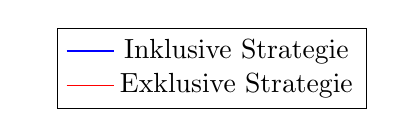
\begin{tikzpicture}
			\begin{axis}[
			width=0.87\textwidth,
			height=0.2\textwidth,
			%		xlabel={Tests (IS)},
			hide axis,
			symbolic x coords={0}
			]
			
			% cycle
			\addplot +[mark=] coordinates {
				(0,0)
			};
			% Load
			\addplot +[mark=] coordinates {
				(0,0)
			};
			% Store
			\addplot +[mark=] coordinates {
				(0,0)
			};
			\legend{Inklusive Strategie, Exklusive Strategie}
			\end{axis}
			\end{tikzpicture}
		\end{minipage}
		\begin{minipage}{0.325\textwidth}
			% IS
			\begin{tikzpicture}
			\begin{semilogyaxis}[
			width=1.15\textwidth,
			xlabel={Tests (IS)},
			legend style={at={(0.5,1.05)},anchor=south},
			symbolic x coords={79, 80, 81, 82, 83, 84, 85, 86}
			]
			
			% inclusiv
			\addplot +[mark=] coordinates {
				(79, 50617585) (80, 50465035) (81, 52132224) (82, 41708585) (83, 22660009) (84, 22916748) (85, 22811790) (86, 22660009)
			};
			% exclusiv
			\addplot +[mark=] coordinates {
				(79, 34896112) (80, 31484235) (81, 24788262) (82, 31034653) (83, 25894023) (84, 25230307) (85, 24911442) (86, 25894023) 
			};
			
			
			%		\legend{a, b, c}
			\end{semilogyaxis}
			\end{tikzpicture}
		\end{minipage}
		%DT
		\begin{minipage}{0.325\textwidth}	
			\begin{tikzpicture}
			\begin{semilogyaxis}[
			width=1.15\textwidth,
			xlabel={Tests (DT)},
			legend style={at={(0.5,1.05)},anchor=south,legend},
			symbolic x coords={79, 80, 81, 82, 83, 84, 85, 86}
			]
			% inclusiv
			\addplot +[mark=] coordinates {
				(79, 2216845) (80, 2312995) (81, 2426046) (82, 2122934) (83, 2126110) (84, 2203558) (85, 2388962) (86, 2126110) 
			};
			% exclusiv
			\addplot +[mark=] coordinates {
				(79, 1966208) (80, 2050492) (81, 2086301) (82, 1963645) (83, 2461961) (84, 2410293) (85, 2563874) (86, 2461961)
			};
			
			%		\legend{Takte, Load, Store}
			\end{semilogyaxis}
			\end{tikzpicture}
		\end{minipage}
		% CG
		\begin{minipage}{0.325\textwidth}
			\begin{tikzpicture}
			\begin{semilogyaxis}[
			width=1.15\textwidth,
			xlabel={Tests (CG)},
			legend style={at={(0.5,1.05)},anchor=south,legend
				columns=-1},
			symbolic x coords={79, 80, 81, 82, 83, 84, 85, 86}
			]
			% inclusiv
			\addplot +[mark=] coordinates {
				(79, 281861317) (80, 253046064) (81, 285023162) (82, 90994546) (83, 91800314) (84, 88307720) (85, 88526507) (86, 91708040)
			};
			% exclusiv
			\addplot +[mark=] coordinates {
				(79, 129645476) (80, 96242016) (81, 93795705) (82, 92430244) (83, 107873591) (84, 96351507) (85, 96421277) (86, 107856802) 
			};
			
			%		\legend{}
			\end{semilogyaxis}
			\end{tikzpicture}
		\end{minipage}
		\caption[Cache-Hierarchie]{Erst f\"ur gro\ss{}e \textit{Caches} (Test 83 - 86) lohnt sich eine inklusive Strategie}
	\end{figure}
}

\subsection{Auswertung}
\frame{\frametitle{Auswertung}
	\begin{block}{Beispiel: optimaler Cache}
	\begin{table}[hbtp]
		\centering
		\begin{tabular}{lc}	
			\tabitem Schreibstrategie: & Write-Back mit Write-Allocate \\
			\pause
			\tabitem Cache-Line Gr\"o\ss{}e: & 64 Byte \\
			\pause
			\tabitem Assoziativit\"at: & 16x Satz-Assoziativ \\
			\pause
			\tabitem Cache Gr\"o\ss{}e: & \begin{tabular}{c}
				L1: 4 KByte 
				\\
				L2: 8 KByte	
			\end{tabular} \\
			\pause
			\tabitem Zugriffszeit: & Niedrig \\
			\pause
			\tabitem Cache-Hierarchie: & Exklusiv \\
		\end{tabular}	
		
	\end{table}

	\end{block}	
}
\frame{\frametitle{Auswertung}
	\begin{figure}[htbp]
		\begin{minipage}{1\textwidth}	
			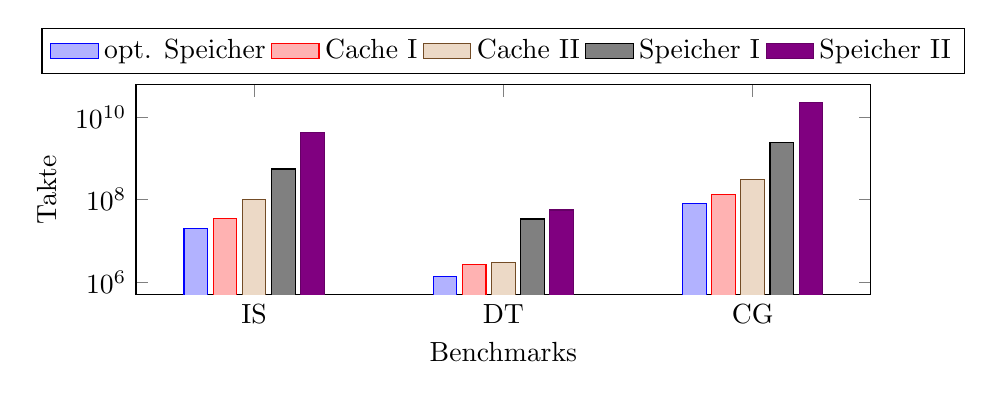
\begin{tikzpicture}
			\begin{semilogyaxis}[
			width=0.9\textwidth,
			enlarge x limits={abs=1.5cm},
			height=0.35\textwidth,
			ybar,
			bar width=0.3cm,
			ylabel={Takte},
			xlabel={Benchmarks},
			legend style={at={(0.5,1.05)},anchor=south,legend
			columns=-1},
			symbolic x coords={IS, DT, CG},
			xtick align=inside,
			xtick=data
			]
			
			% opt mem
			\addplot +[area legend] coordinates {
				(IS, 19561595)	
				(DT, 1335536)
				(CG, 82305441)
				
			};
			
			% cache with no collisions
			\addplot +[area legend] coordinates {
				%			(IS, 24763281)	
				(IS, 34233977)
				%			(DT, 1832087)
				(DT, 2690141)
				%			(CG, 116606189)
				(CG, 132061379)
			};
			
			% cache
			\addplot +[area legend] coordinates {
				%			(IS, 35576931)	
				(IS, 99460615)
				%			(DT, 1966997)
				(DT, 2987284)
				%			(CG, 136512409)
				(CG, 309661917)
				
			};
			% mem with no collisions
			\addplot +[area legend] coordinates {
				(IS, 557993495)	
				(DT, 34027835)
				(CG, 2412080710)
				
			};
			
			% mem
			\addplot +[area legend] coordinates {
				(IS, 4237672597)	
				(DT, 56306471)
				(CG, 23268927312)
				
			};		
			\legend{opt. Speicher,
				Cache I,
				Cache II,
				Speicher I,
				Speicher II
			}
			\end{semilogyaxis}
			\end{tikzpicture}
		\end{minipage}
		
		\caption[Speichersysteme]{Ausf\"uhrungszeit mit unterschiedlichen Speichersystemen.}
	\end{figure}
}
\frame{\frametitle{Auswertung}
	\begin{figure}[htbp]
		\begin{minipage}{1\textwidth}	
			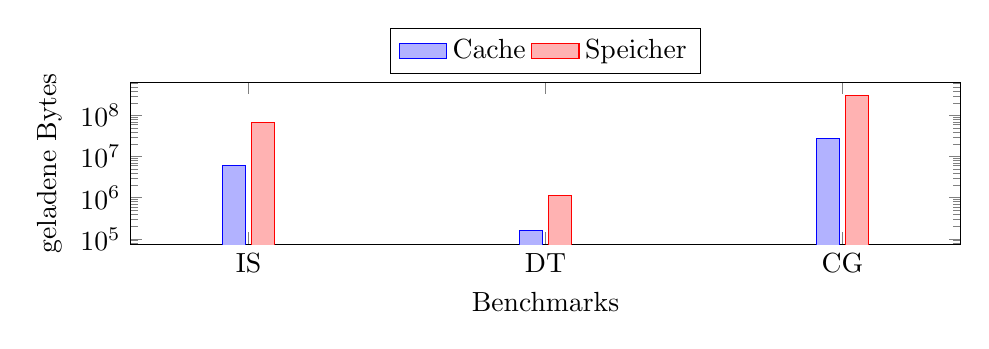
\begin{tikzpicture}
			\begin{semilogyaxis}[
			width=1\textwidth,
			enlarge x limits={abs=1.5cm},
			height=0.3\textwidth,
			ybar,
			bar width=0.3cm,
			ylabel={geladene Bytes},
			xlabel={Benchmarks},
			legend style={at={(0.5,1.05)},anchor=south,legend
				columns=-1},
			symbolic x coords={IS, DT, CG},
			xtick align=inside,
			xtick=data
			]
			% cache
			\addplot +[area legend] coordinates {
				%			(IS, 2553792)	
				(IS, 5995520)
				%			(DT, 89216)
				(DT, 156992)
				%			(CG, 19424384)
				(CG, 27899008)
				
			};
			% mem
			\addplot +[area legend] coordinates {
				(IS, 67793976)	
				(DT, 1157136)
				(CG, 301377384)
				
			};		
			\legend{Cache,
				Speicher
			}
			\end{semilogyaxis}
			\end{tikzpicture}
		\end{minipage}
		\begin{minipage}{1\textwidth}	
			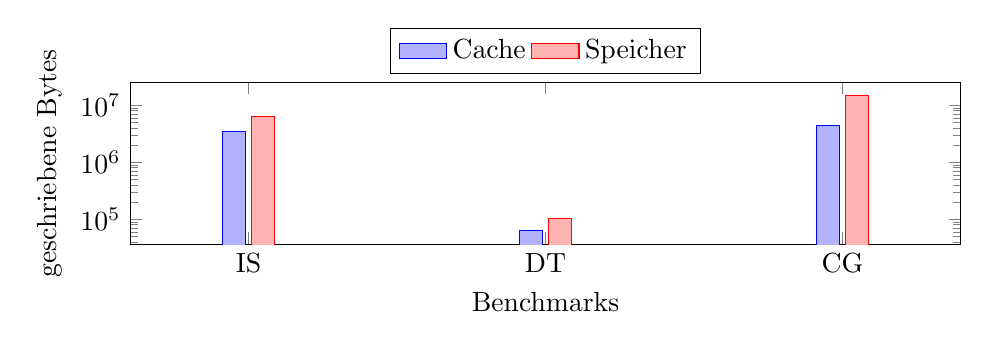
\begin{tikzpicture}
			\begin{semilogyaxis}[
			width=1\textwidth,
			enlarge x limits={abs=1.5cm},
			height=0.3\textwidth,
			ybar,
			bar width=0.3cm,
			ylabel={geschriebene Bytes},
			xlabel={Benchmarks},
			legend style={at={(0.5,1.05)},anchor=south,legend
				columns=-1},
			symbolic x coords={IS, DT, CG},
			xtick align=inside,
			xtick=data
			]
			% cache
			\addplot +[area legend] coordinates {
				%			(IS, 632384)
				(IS, 3494592)	
				%			(DT, 1088)
				(DT, 62592)
				%			(CG, 4203840)
				(CG, 4475200)
				
			};
			% mem
			\addplot +[area legend] coordinates {
				(IS, 6247136)	
				(DT, 102504)
				(CG, 14568112)
				
			};		
			\legend{Cache,
				Speicher
			}
			\end{semilogyaxis}
			\end{tikzpicture}
		\end{minipage}
		
		\caption[Speichersysteme]{Traffic mit unterschiedlichen Speichersystemen.}
	\end{figure}
}
\frame{\frametitle{Auswertung}
\begin{figure}[htbp]
	\begin{table}[hbtp]
		\begin{tabular}{c|c|c|c}
			- & IS & DT & CG \\\hline
			I & 	
			\begin{minipage}{0.3\textwidth}
				\includegraphics[width=1\textwidth,height=0.49\textwidth]{exec_timeline/is_cache.png}
			\end{minipage} &
			\begin{minipage}{0.3\textwidth}
				\includegraphics[width=1\textwidth,height=0.49\textwidth]{exec_timeline/dt_cache.png}
			\end{minipage} &
			\begin{minipage}{0.3\textwidth}
				\includegraphics[width=1\textwidth,height=0.49\textwidth]{exec_timeline/cg_cache.png}
			\end{minipage}
			
			\\\hline
			II & 	
			\begin{minipage}{0.3\textwidth}
				\includegraphics[width=1\textwidth,height=0.49\textwidth]{exec_timeline/is_no_cache.png}
			\end{minipage} &
			\begin{minipage}{0.3\textwidth}
				\includegraphics[width=1\textwidth,height=0.49\textwidth]{exec_timeline/dt_no_cache.png}
			\end{minipage} &
			\begin{minipage}{0.3\textwidth}
				\includegraphics[width=1\textwidth,height=0.49\textwidth]{exec_timeline/cg_no_cache.png}
			\end{minipage}
			
			\\\hline
		\end{tabular}
	\end{table}

	
	\caption[Programmablauf]{Programmablauf auf verschiedenen Systemen (I: mit Cache | II: ohne Cache)}
	\label{f:execTimeFlow}
\end{figure}	
}
\section{Fazit}
\frame{\frametitle{Fazit}
	\begin{block}{Vorteile}
		\tabitem K\"urzere Ausf\"uhrungszeit\\
		\tabitem Seltenere RAM-Zugriffe\\
		\tabitem Weniger Gesamt-Traffic
	\end{block}	
	\pause
	\begin{block}{Nachteile}
		\tabitem H\"oherer Traffic relativ zur Ausf\"uhrungszeit\\
		\tabitem Schlechtere Echtzeitf\"ahigkeit
	\end{block}	
	\pause
	\begin{block}{Unterschiede zu anderen Architekturen}
		\tabitem Kleinere Caches\\
		\tabitem Exklusiv\\
		\tabitem Kein getrennter Instruction-Cache
	\end{block}		
	
}
\end{document}
